\documentclass[aspectratio=169, 10pt]{beamer}

% ==============================================================================
% PACKAGES & THEME CONFIGURATION
% ==============================================================================
\usetheme{Madrid}
\usecolortheme{default}
\usefonttheme{professionalfonts}

\usepackage[utf8]{inputenc}
\usepackage[T1]{fontenc}
\usepackage{lmodern}
\usepackage{graphicx}
\usepackage{booktabs}
\usepackage{tabularx}
\usepackage{array}
\usepackage{amsmath, amssymb}
\usepackage{tikz}
\usetikzlibrary{arrows.meta, positioning, shapes.geometric, shapes.multipart, fit, backgrounds, calc}
\usepackage{xcolor}
\usepackage{hyperref}

% ==============================================================================
% COLOR PALETTE (Academic Navy, Biotech Teal & Gold)
% ==============================================================================
\definecolor{navyprimary}{RGB}{20, 48, 88}
\definecolor{steelsecondary}{RGB}{38, 102, 163}
\definecolor{biotechteal}{RGB}{16, 124, 120}
\definecolor{amberaccent}{RGB}{196, 122, 24}
\definecolor{crimsonalert}{RGB}{178, 34, 52}
\definecolor{cardbg}{RGB}{244, 247, 252}
\definecolor{tealbg}{RGB}{238, 248, 247}
\definecolor{amberbg}{RGB}{253, 247, 236}
\definecolor{slateborder}{RGB}{205, 216, 230}
\definecolor{textdark}{RGB}{32, 38, 46}
\definecolor{textmuted}{RGB}{90, 102, 118}

\setbeamercolor{palette primary}{bg=navyprimary, fg=white}
\setbeamercolor{palette secondary}{bg=steelsecondary, fg=white}
\setbeamercolor{palette tertiary}{bg=biotechteal, fg=white}
\setbeamercolor{palette quaternary}{bg=navyprimary, fg=white}
\setbeamercolor{structure}{fg=navyprimary}
\setbeamercolor{frametitle}{bg=navyprimary, fg=white}
\setbeamercolor{title}{fg=navyprimary}
\setbeamercolor{normal text}{fg=textdark, bg=white}
\setbeamercolor{block title}{bg=navyprimary, fg=white}
\setbeamercolor{block body}{bg=cardbg, fg=textdark}
\setbeamercolor{block title example}{bg=biotechteal, fg=white}
\setbeamercolor{block body example}{bg=tealbg, fg=textdark}
\setbeamercolor{block title alerted}{bg=amberaccent, fg=white}
\setbeamercolor{block body alerted}{bg=amberbg, fg=textdark}
\setbeamercolor{itemize item}{fg=steelsecondary}
\setbeamercolor{itemize subitem}{fg=biotechteal}
\setbeamercolor{enumerate item}{fg=navyprimary}

\setbeamertemplate{navigation symbols}{}
\setbeamertemplate{blocks}[rounded][shadow=false]
\setbeamertemplate{itemize items}[circle]
\setbeamertemplate{itemize subitem}[triangle]

% Custom Footline
\setbeamertemplate{footline}{
  \leavevmode%
  \hbox{%
  \begin{beamercolorbox}[wd=.38\paperwidth,ht=2.4ex,dp=1ex,left,leftskip=1em]{author in head/foot}%
    \usebeamerfont{author in head/foot}Aradhya Gupta (SAU) $\cdot$ Prof.\ Arindam Mondal Lab (IIT KGP)
  \end{beamercolorbox}%
  \begin{beamercolorbox}[wd=.44\paperwidth,ht=2.4ex,dp=1ex,center]{title in head/foot}%
    \usebeamerfont{title in head/foot}DDX3X--Influenza B Virus Genomic RNA Interaction
  \end{beamercolorbox}%
  \begin{beamercolorbox}[wd=.18\paperwidth,ht=2.4ex,dp=1ex,right,rightskip=1em]{date in head/foot}%
    \usebeamerfont{date in head/foot}Slide \insertframenumber{} / \inserttotalframenumber
  \end{beamercolorbox}}%
  \vskip0pt%
}

% Custom Frame Title
\setbeamertemplate{frametitle}{
  \nointerlineskip%
  \begin{beamercolorbox}[wd=\paperwidth,ht=2.8ex,dp=1.1ex,leftskip=1.2em]{frametitle}%
    \usebeamerfont{frametitle}\textbf{\insertframetitle}%
    \ifx\insertframesubtitle\@empty\else%
      \hfill{\small\color{white!80}\insertframesubtitle}%
    \fi%
  \end{beamercolorbox}%
  \nointerlineskip%
  {\color{amberaccent}\hrule height 1.5pt}%
}

% Helper macro for clean bordered figure boxes
\newcommand{\figbox}[2][]{%
  \begin{tikzpicture}
    \node[draw=slateborder, line width=0.6pt, rounded corners=3pt, inner sep=3pt, fill=white] {\includegraphics[#1]{#2}};
  \end{tikzpicture}%
}

% Metadata
\title[DDX3X--IBV RNA Interaction]{Characterization of the Interaction Between DDX3X and Influenza B Virus Genomic RNA}
\subtitle{Final Internship Report}
\author[Aradhya Gupta]{Aradhya Gupta}
\institute[SAU / IIT Kharagpur]{1st Year BS-MS, South Asian University \\ Supervised by Prof.\ Arindam Mondal, Dept.\ of Bioscience and Biotechnology, IIT Kharagpur}
\date{}

\begin{document}

% ==============================================================================
% SLIDE 1: TITLE SLIDE
% ==============================================================================
{
\setbeamertemplate{footline}{}
\begin{frame}[plain]
  \begin{tikzpicture}[remember picture, overlay]
    % Top accent bar
    \fill[navyprimary] (current page.north west) rectangle ([yshift=-0.22cm]current page.north east);
    \fill[amberaccent] ([yshift=-0.22cm]current page.north west) rectangle ([yshift=-0.30cm]current page.north east);
    % Subtle bottom bar
    \fill[cardbg] (current page.south west) rectangle ([yshift=1.15cm]current page.south east);
    \draw[slateborder, line width=0.8pt] ([yshift=1.15cm]current page.south west) -- ([yshift=1.15cm]current page.south east);
  \end{tikzpicture}

  \vspace{0.2cm}
  \begin{columns}[c]
    \begin{column}{0.16\textwidth}
      \centering
      
\includegraphics[height=1.85cm]{figures_opt/image2.png}
    \end{column}
    \begin{column}{0.68\textwidth}
      \centering
      {\small\bfseries\color{biotechteal}\MakeUppercase{Final Internship Report}}
    \end{column}
    \begin{column}{0.16\textwidth}
      \centering
      
\includegraphics[height=1.85cm]{figures_opt/image3.png}
    \end{column}
  \end{columns}

  \vspace{0.35cm}
  \begin{center}
    \begin{beamercolorbox}[wd=0.92\textwidth, rounded=true, shadow=false, sep=1.1em, center]{block body}
      {\LARGE\bfseries\color{navyprimary} Characterization of the Interaction Between DDX3X and Influenza B Virus Genomic RNA}
    \end{beamercolorbox}
  \end{center}

  \vspace{0.45cm}
  \begin{columns}[T]
    \begin{column}{0.46\textwidth}
      \centering
      {\footnotesize\color{textmuted}\textbf{SUBMITTED BY}}\\[0.25em]
      {\large\bfseries\color{navyprimary} Aradhya Gupta}\\[0.15em]
      {\small\color{textdark} 1st Year BS-MS}\\
      {\small\color{steelsecondary} South Asian University}
    \end{column}
    \begin{column}{0.04\textwidth}
      \centering
      \color{slateborder}\rule{0.8pt}{1.8cm}
    \end{column}
    \begin{column}{0.48\textwidth}
      \centering
      {\footnotesize\color{textmuted}\textbf{UNDER THE SUPERVISION OF}}\\[0.25em]
      {\large\bfseries\color{navyprimary} Prof.\ Arindam Mondal}\\[0.15em]
      {\small\color{textdark} Molecular Virology Laboratory}\\
      {\small\color{steelsecondary} Dept.\ of Bioscience and Biotechnology, IIT Kharagpur}
    \end{column}
  \end{columns}
\end{frame}
}

% ==============================================================================
% SLIDE 2: INFLUENZA: A MAJOR CONCERN FOR PUBLIC HEALTH
% ==============================================================================
\begin{frame}{Influenza: A Major Concern for Public Health}
  \begin{columns}[T]
    \begin{column}{0.41\textwidth}
      \begin{block}{Epidemiology \& Classification}
        \small
        \begin{itemize}
          \item Belongs to family \textbf{Orthomyxoviridae}; causes acute respiratory infections.
          \item Drives seasonal epidemics causing \textbf{3 to 5 million} severe infections annually worldwide.
          \item Segmented negative-sense ssRNA genome enables rapid antigenic evolution.
        \end{itemize}
      \end{block}
      \vspace{0.15cm}
      \begin{alertblock}{Public Health Impact}
        \footnotesize High mutation rates and segmented genomes necessitate continuous surveillance and host-factor targeted antiviral research.
      \end{alertblock}
    \end{column}

    \begin{column}{0.56\textwidth}
      \begin{block}{Types of Influenza Virus}
        \renewcommand{\arraystretch}{1.2}
        \footnotesize
        \begin{tabularx}{\linewidth}{@{}l l X@{}}
          \toprule
          \textbf{Type} & \textbf{Primary Hosts} & \textbf{Clinical \& Epidemiological Significance} \\
          \midrule
          \textbf{Influenza A} & Birds \& Mammals & Caused \textbf{4 pandemics} (1918--2009: H1N1, H2N2, H3N2). \\
          \textbf{Influenza B} & \textbf{Exclusively Humans} & Causes seasonal flu outbreaks; major pediatric burden. \\
          \textbf{Influenza C} & Humans \& Pigs & Primarily causes mild upper respiratory illness. \\
          \textbf{Influenza D} & Cattle \& Pigs & Newly proposed genus; not known to infect humans. \\
          \bottomrule
        \end{tabularx}
      \end{block}
      \vspace{0.15cm}
      {\scriptsize\color{textmuted}\textbf{Reference:} \textit{Molecular Medical Microbiology}. DOI: \href{https://doi.org/10.1016/B978-0-12-818619-0.00093-9}{10.1016/B978-0-12-818619-0.00093-9}}
    \end{column}
  \end{columns}
\end{frame}

% ==============================================================================
% SLIDE 3: STRUCTURE OF INFLUENZA VIRUS
% ==============================================================================
\begin{frame}{Structure of Influenza Virus}
  \begin{columns}[c]
    \begin{column}{0.49\textwidth}
      \begin{block}{Virion \& Genomic Organization}
        \small
        \begin{itemize}
          \item Negative-sense, single-stranded RNA virus.
          \item Enveloped virion decorated with surface glycoproteins (\textbf{HA}, \textbf{NA}) and \textbf{M2} ion channel, lined internally by \textbf{M1}.
          \item \textbf{8 segments} of negative-sense viral RNA (vRNA) packaged as \textbf{Ribonucleoprotein Complexes (vRNPs)}.
          \item \textbf{Oligomeric NP} binds vRNA non-specifically.
          \item \textbf{RNA-dependent RNA Polymerase (PB1+PB2+PA)} binds the conserved $5'$ and $3'$ viral promoter region.
          \item Self-sufficient machinery for viral RNA synthesis: \textbf{transcription} and \textbf{replication}.
        \end{itemize}
      \end{block}
    \end{column}

    \begin{column}{0.49\textwidth}
      \centering
      \textbf{\small\color{navyprimary} Virion Architecture \& RNP Complex}\\[0.2em]
      \figbox[width=0.84\linewidth, height=4.6cm, keepaspectratio]{figures_opt/image4.png}\\[0.2em]
      {\scriptsize\color{textmuted} Surface glycoproteins (HA, NA, M2), M1 matrix shell, and 8 vRNP segments (PB1, PB2, PA, NP+vRNA, $5'/3'$ promoter).}
    \end{column}
  \end{columns}
\end{frame}

% ==============================================================================
% SLIDE 4: LIFE CYCLE OF INFLUENZA VIRUS
% ==============================================================================
\begin{frame}{Life Cycle of Influenza Virus}
  \begin{columns}[c]
    \begin{column}{0.44\textwidth}
      \begin{block}{Key Stages of Viral Infection}
        \footnotesize
        \begin{enumerate}
          \setlength\itemsep{0.25em}
          \item \textbf{Attachment:} Hemagglutinin (HA) binds host sialic acid receptors, triggering endocytosis.
          \item \textbf{Fusion \& Uncoating:} Endosomal acidification induces membrane fusion and releases vRNPs into cytoplasm.
          \item \textbf{Nuclear Import:} vRNPs are actively imported into the host nucleus.
          \item \textbf{Transcription \& Replication:} Viral RdRp synthesizes mRNA ($\text{vRNA}(-) \rightarrow \text{mRNA}(+)$) and replicates genome ($\text{vRNA} \rightarrow \text{cRNA} \rightarrow \text{vRNA}$).
          \item \textbf{Translation \& RNP Export:} Viral proteins are translated; progeny vRNPs exit the nucleus.
          \item \textbf{Assembly, Budding \& Release:} Progeny virions assemble at plasma membrane; NA facilitates release.
        \end{enumerate}
      \end{block}
    \end{column}

    \begin{column}{0.54\textwidth}
      \centering
      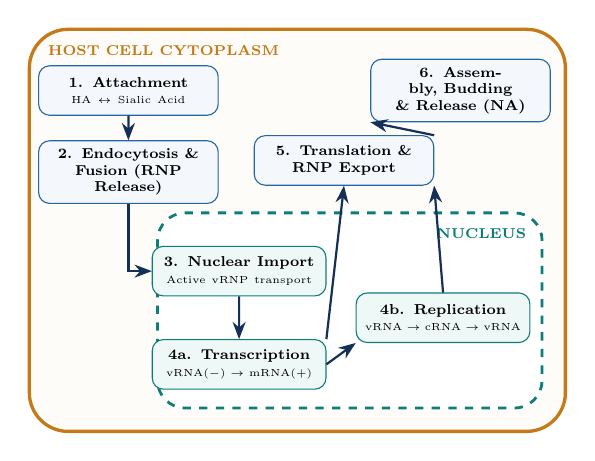
\begin{tikzpicture}[
        scale=0.74, transform shape,
        stage/.style={draw=steelsecondary, fill=cardbg, rounded corners=4pt, text width=2.8cm, align=center, font=\scriptsize\bfseries, inner sep=4pt, minimum height=0.85cm},
        nuc/.style={draw=biotechteal, fill=tealbg, rounded corners=4pt, text width=2.7cm, align=center, font=\scriptsize\bfseries, inner sep=4pt, minimum height=0.85cm},
        arr/.style={-{Stealth[length=2.2mm]}, thick, navyprimary}
      ]
        % Cell boundary
        \draw[draw=amberaccent, fill=amberbg!35, rounded corners=14pt, line width=1.2pt] (-0.4,-0.4) rectangle (8.8,6.5);
        \node[anchor=north west, font=\scriptsize\bfseries\color{amberaccent}] at (-0.2,6.35) {HOST CELL CYTOPLASM};

        % Nucleus boundary
        \draw[draw=biotechteal, dashed, fill=white, rounded corners=10pt, line width=1pt] (1.8,0.0) rectangle (8.4,3.35);
        \node[anchor=north east, font=\scriptsize\bfseries\color{biotechteal}] at (8.25,3.2) {NUCLEUS};

        % Nodes
        \node[stage] (att) at (1.3, 5.45) {1. Attachment\\{\normalfont\tiny HA $\leftrightarrow$ Sialic Acid}};
        \node[stage] (end) at (1.3, 4.05) {2. Endocytosis \&\\Fusion (RNP Release)};
        \node[nuc]   (imp) at (3.2, 2.35) {3. Nuclear Import\\{\normalfont\tiny Active vRNP transport}};
        \node[nuc]   (tx)  at (3.2, 0.75) {4a. Transcription\\{\normalfont\tiny $\text{vRNA}(-) \rightarrow \text{mRNA}(+)$}};
        \node[nuc]   (rep) at (6.7, 1.55) {4b. Replication\\{\normalfont\tiny $\text{vRNA} \rightarrow \text{cRNA} \rightarrow \text{vRNA}$}};
        \node[stage] (trl) at (5.0, 4.25) {5. Translation \&\\RNP Export};
        \node[stage] (bud) at (7.0, 5.45) {6. Assembly, Budding\\\& Release (NA)};

        % Arrows
        \draw[arr] (att) -- (end);
        \draw[arr] (end) |- (imp);
        \draw[arr] (imp) -- (tx);
        \draw[arr] (tx.east) -- (rep.south west);
        \draw[arr] (tx.north east) -- (trl.south);
        \draw[arr] (rep.north) -- (trl.south east);
        \draw[arr] (trl.north east) -- (bud.south west);
      \end{tikzpicture}
    \end{column}
  \end{columns}
\end{frame}

% ==============================================================================
% SLIDE 5: HOST PROTEINS & INFLUENZA vRNP SYNTHESIS
% ==============================================================================
\begin{frame}{Host Factors Modulating Influenza vRNP Synthesis}
  \begin{center}
    \begin{alertblock}{}
      \centering\bfseries Various host proteins influence the synthesis of Influenza virus RNPs and affect the viral life cycle.
    \end{alertblock}
  \end{center}

  \vspace{0.15cm}
  \begin{center}
    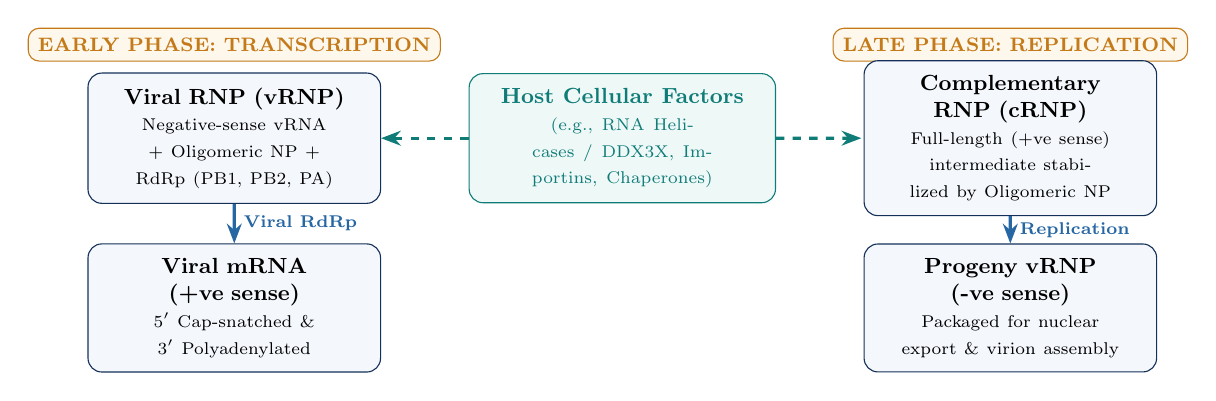
\begin{tikzpicture}[
      scale=0.88, transform shape,
      box/.style={draw=navyprimary, fill=cardbg, rounded corners=5pt, text width=3.8cm, align=center, inner sep=6pt, font=\small},
      phase/.style={draw=amberaccent, fill=amberbg, rounded corners=4pt, font=\footnotesize\bfseries\color{amberaccent}, inner sep=4pt},
      host/.style={draw=biotechteal, fill=tealbg, rounded corners=5pt, text width=4.0cm, align=center, inner sep=6pt, font=\small\bfseries\color{biotechteal}},
      arr/.style={-{Stealth[length=2.5mm]}, very thick, steelsecondary}
    ]
      % Early Phase
      \node[phase] (ep) at (0, 3.8) {EARLY PHASE: TRANSCRIPTION};
      \node[box] (vrnp1) at (0, 2.45) {\textbf{Viral RNP (vRNP)}\\{\scriptsize Negative-sense vRNA + Oligomeric NP + RdRp (PB1, PB2, PA)}};
      \node[box] (mrna) at (0, 0.0) {\textbf{Viral mRNA (+ve sense)}\\{\scriptsize $5'$ Cap-snatched \& $3'$ Polyadenylated}};
      \draw[arr] (vrnp1) -- node[right, font=\scriptsize\bfseries\color{textdark}] {Viral RdRp} (mrna);

      % Host Factor Bridge
      \node[host] (hf) at (5.6, 2.45) {Host Cellular Factors\\{\normalfont\scriptsize (e.g., RNA Helicases / DDX3X, Importins, Chaperones)}};
      \draw[arr, biotechteal, dashed] (hf.west) -- (vrnp1.east);
      \draw[arr, biotechteal, dashed] (hf.east) -- (9.05, 2.45);

      % Late Phase
      \node[phase] (lp) at (11.2, 3.8) {LATE PHASE: REPLICATION};
      \node[box] (crnp) at (11.2, 2.45) {\textbf{Complementary RNP (cRNP)}\\{\scriptsize Full-length (+ve sense) intermediate stabilized by Oligomeric NP}};
      \node[box] (vrnp2) at (11.2, 0.0) {\textbf{Progeny vRNP (-ve sense)}\\{\scriptsize Packaged for nuclear export \& virion assembly}};
      \draw[arr] (crnp) -- node[right, font=\scriptsize\bfseries\color{textdark}] {Replication} (vrnp2);
    \end{tikzpicture}
  \end{center}
\end{frame}

% ==============================================================================
% SLIDE 6: HUMAN DEAD-BOX RNA HELICASE 3 X-LINKED (DDX3X)
% ==============================================================================
\begin{frame}{Human DEAD-Box RNA Helicase 3 X-Linked (DDX3X)}
  \begin{columns}[T]
    \begin{column}{0.48\textwidth}
      \begin{block}{Cellular RNA Metabolism}
        \begin{itemize}
          \item \textbf{DDX3X} is a conserved DEAD-box ATP-dependent RNA helicase (Superfamily 2).
          \item Regulates multiple facets of RNA metabolism:
            \begin{itemize}
              \item RNA duplex unwinding
              \item mRNA nuclear export
              \item Translation initiation
              \item Ribonucleoprotein (RNP) complex remodelling
            \end{itemize}
          \item As an RNA-binding protein, DDX3X governs cellular gene expression pathways.
        \end{itemize}
      \end{block}
    \end{column}

    \begin{column}{0.48\textwidth}
      \begin{exampleblock}{Antiviral Innate Immunity}
        \begin{itemize}
          \item Key component of the host innate immune response against viral pathogens.
          \item Enhances \textbf{Type I Interferon ($\text{IFN}-\alpha/\beta$)} signaling via TBK1/IKK$\varepsilon$--IRF3 pathways.
          \item Promotes transcription of antiviral interferon-stimulated genes (ISGs).
        \end{itemize}
      \end{exampleblock}
      \vspace{0.25cm}
      \begin{alertblock}{Multifunctional Host Factor}
        \small Its dual role in RNA metabolism and antiviral signaling makes DDX3X a critical host factor during influenza virus infection.
      \end{alertblock}
    \end{column}
  \end{columns}
\end{frame}

% ==============================================================================
% SLIDE 7: STRUCTURE OF DDX3X
% ==============================================================================
\begin{frame}{Structure of DDX3X (DEAD-Box Helicase 3 X-Linked)}
  \begin{columns}[c]
    \begin{column}{0.60\textwidth}
      \centering
      \figbox[width=0.95\linewidth, height=5.2cm, keepaspectratio]{figures_opt/image23.png}
    \end{column}
    \begin{column}{0.38\textwidth}
      \begin{block}{Structural Architecture}
        \footnotesize
        \begin{itemize}
          \item \textbf{Helicase Core:} Two conserved RecA-like domains (Domain 1 \& Domain 2) connected by a flexible linker.
          \item \textbf{Catalytic Motifs:} Contains the signature \textbf{D-E-A-D} (Asp-Glu-Ala-Asp) Walker B motif and Walker A P-loop for ATP binding and hydrolysis.
          \item \textbf{RNA-Binding Cleft:} Formed across the inter-domain interface to engage single-stranded RNA.
          \item \textbf{N- \& C-Terminal Extensions:} Mediate protein--protein interactions and subcellular localization.
        \end{itemize}
      \end{block}
    \end{column}
  \end{columns}
\end{frame}

% ==============================================================================
% SLIDE 8: BACKGROUND STUDY
% ==============================================================================
\begin{frame}{Background Study}
  \begin{columns}[c]
    \begin{column}{0.38\textwidth}
      \centering
      \figbox[width=0.88\linewidth, height=5.4cm, keepaspectratio]{figures_opt/image24.png}\\[0.2em]
      {\scriptsize\color{textmuted}\textit{Data generated by Mr.\ Soumik Dey (Mondal Lab)}}
    \end{column}

    \begin{column}{0.59\textwidth}
      \begin{block}{Previous Laboratory Findings}
        \begin{itemize}
          \item DDX3X \textbf{selectively downregulates} viral RNA synthesis in \textbf{Influenza B virus (IBV)} in a dose-dependent manner ($p < 0.0001$).
          \item Conversely, \textbf{no inhibitory effect} was observed during \textbf{Influenza A virus (IAV)} infection when interacting with both viral promoter regions (UTRs).
        \end{itemize}
      \end{block}
      \vspace{0.3cm}
      \begin{alertblock}{Unresolved Research Question}
        \textbf{Does DDX3X interact with all eight genomic RNA segments of Influenza B virus, or only a specific subset of them?}
      \end{alertblock}
    \end{column}
  \end{columns}
\end{frame}

% ==============================================================================
% SLIDE 9: OBJECTIVES
% ==============================================================================
\begin{frame}{Project Objectives}
  \begin{columns}[c]
    \begin{column}{0.56\textwidth}
      \begin{block}{Specific Aims of the Internship}
        \begin{enumerate}
          \setlength\itemsep{0.8em}
          \item \textbf{Protein Expression \& Purification:}\\
          Expression and purification of recombinant human DDX3X protein in \textit{E.\ coli} BL21(DE3) host cells.
          \item \textbf{In Vitro Viral RNA Generation:}\\
          Generation of different genomic RNA segments (mini-viral constructs) of Influenza B virus \textit{in vitro}.
          \item \textbf{RNA--Protein Interaction Characterization:}\\
          Characterizing the direct interaction between purified DDX3X and individual Influenza B virus genomic RNA segments \textit{in vitro}.
        \end{enumerate}
      \end{block}
    \end{column}

    \begin{column}{0.41\textwidth}
      \centering
      \figbox[width=0.95\linewidth, height=5.2cm, keepaspectratio]{figures_opt/image25.jpeg}
    \end{column}
  \end{columns}
\end{frame}

% ==============================================================================
% SLIDE 10: OBJECTIVE 1 - METHODOLOGY
% ==============================================================================
\begin{frame}{Objective 1: Protein Expression and Purification}
  \framesubtitle{Methodology}
  \begin{columns}[T]
    \begin{column}{0.48\textwidth}
      \begin{block}{Expression \& Cell Harvesting}
        \small
        \begin{itemize}
          \item Recombinant His-tagged human DDX3X was expressed in \textit{E.\ coli} \textbf{BL21(DE3)} host cells following \textbf{IPTG induction}.
          \item Large-scale bacterial culture expression performed under optimized temperature and induction conditions.
          \item Cells harvested by centrifugation and lysed via sonication in lysis buffer to release soluble protein.
        \end{itemize}
      \end{block}
    \end{column}

    \begin{column}{0.48\textwidth}
      \begin{exampleblock}{Chromatographic Purification \& QC}
        \small
        \begin{itemize}
          \item \textbf{Ni-NTA Affinity Chromatography:} Captured His-tagged DDX3X and collected imidazole elution fractions (E1--E6).
          \item \textbf{Size Exclusion Chromatography (SEC):} Further polished pooled fractions to isolate monodisperse protein (E11--E19).
          \item \textbf{SDS-PAGE Verification:} Confirmed protein expression, molecular weight ($\sim 73\text{ kDa}$), and purity.
        \end{itemize}
      \end{exampleblock}
    \end{column}
  \end{columns}

  \vspace{0.35cm}
  \begin{center}
    
\begin{tikzpicture}[
      scale=0.92, transform shape,
      stepbox/.style={draw=navyprimary, fill=cardbg, rounded corners=4pt, minimum width=2.15cm, minimum height=0.85cm, align=center, font=\scriptsize\bfseries},
      arr/.style={-{Stealth[length=2mm]}, thick, amberaccent}
    ]
      \node[stepbox] (s1) at (0,0) {BL21(DE3)\\Transformation};
      \node[stepbox] (s2) at (2.9,0) {IPTG\\Induction};
      \node[stepbox] (s3) at (5.8,0) {Harvest \&\\Cell Lysis};
      \node[stepbox] (s4) at (8.7,0) {Ni-NTA\\Affinity};
      \node[stepbox] (s5) at (11.6,0) {SEC \&\\SDS-PAGE};
      \draw[arr] (s1) -- (s2);
      \draw[arr] (s2) -- (s3);
      \draw[arr] (s3) -- (s4);
      \draw[arr] (s4) -- (s5);
    \end{tikzpicture}
  \end{center}
\end{frame}

% ==============================================================================
% SLIDE 11: EXPRESSION ANALYSIS & HIS-TAG PURIFICATION
% ==============================================================================
\begin{frame}{Expression Analysis \& Ni-NTA Purification of DDX3X}
  \begin{columns}[c]
    \begin{column}{0.48\textwidth}
      \begin{block}{IPTG Induction Analysis}
        \begin{itemize}
          \item Distinct overexpressed protein band observed following IPTG induction in \textbf{Lane 3 (IN)}.
          \item Band migrates at the expected molecular weight of recombinant DDX3X (\textbf{$\sim 73\text{ kDa}$}).
        \end{itemize}
      \end{block}
      \vspace{0.15cm}
      \centering
      \begin{tikzpicture}
        \node[draw=slateborder, line width=0.6pt, rounded corners=3pt, inner sep=3pt, fill=white] (g1) {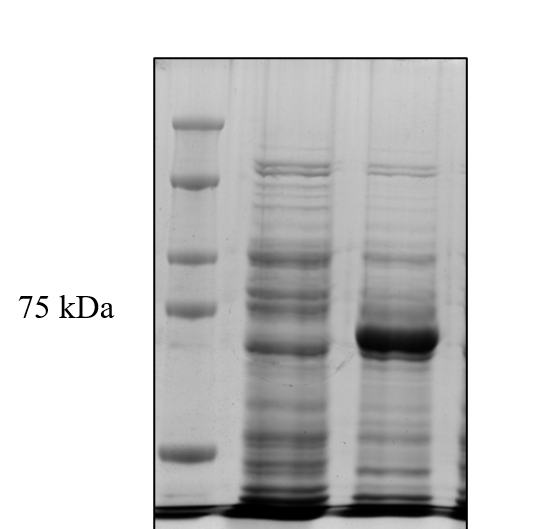
\includegraphics[height=3.4cm, keepaspectratio]{figures_opt/image26.png}};
        \node[anchor=south, font=\scriptsize\bfseries\color{navyprimary}] at ([xshift=-0.85cm, yshift=0.05cm]g1.north) {M};
        \node[anchor=south, font=\scriptsize\bfseries\color{navyprimary}] at ([xshift=0.15cm, yshift=0.05cm]g1.north) {UN};
        \node[anchor=south, font=\scriptsize\bfseries\color{navyprimary}] at ([xshift=1.05cm, yshift=0.05cm]g1.north) {IN};
      \end{tikzpicture}
    \end{column}

    \begin{column}{0.48\textwidth}
      \begin{exampleblock}{His-Tag Affinity Purification}
        \begin{itemize}
          \item Successful capture and elution of His-tagged DDX3X via \textbf{Ni-NTA affinity chromatography}.
          \item Strong enrichment observed across elution fractions \textbf{E1--E6}.
        \end{itemize}
      \end{exampleblock}
      \vspace{0.15cm}
      \centering
      \begin{tikzpicture}
        \node[draw=slateborder, line width=0.6pt, rounded corners=3pt, inner sep=3pt, fill=white] (g2) {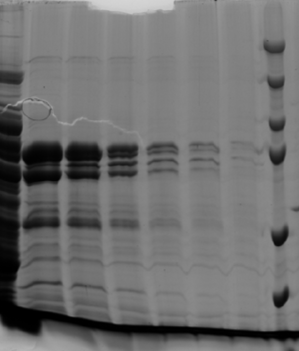
\includegraphics[height=3.4cm, keepaspectratio]{figures_opt/image27.png}};
        \node[anchor=south, font=\tiny\bfseries\color{biotechteal}] at ([xshift=-1.25cm, yshift=0.05cm]g2.north) {IN};
        \node[anchor=south, font=\tiny\bfseries\color{biotechteal}] at ([xshift=-0.90cm, yshift=0.05cm]g2.north) {E1};
        \node[anchor=south, font=\tiny\bfseries\color{biotechteal}] at ([xshift=-0.55cm, yshift=0.05cm]g2.north) {E2};
        \node[anchor=south, font=\tiny\bfseries\color{biotechteal}] at ([xshift=-0.20cm, yshift=0.05cm]g2.north) {E3};
        \node[anchor=south, font=\tiny\bfseries\color{biotechteal}] at ([xshift=0.15cm, yshift=0.05cm]g2.north) {E4};
        \node[anchor=south, font=\tiny\bfseries\color{biotechteal}] at ([xshift=0.50cm, yshift=0.05cm]g2.north) {E5};
        \node[anchor=south, font=\tiny\bfseries\color{biotechteal}] at ([xshift=0.85cm, yshift=0.05cm]g2.north) {E6};
        \node[anchor=south, font=\tiny\bfseries\color{biotechteal}] at ([xshift=1.22cm, yshift=0.05cm]g2.north) {M};
      \end{tikzpicture}
    \end{column}
  \end{columns}
\end{frame}

% ==============================================================================
% SLIDE 12: SIZE EXCLUSION CHROMATOGRAPHY
% ==============================================================================
\begin{frame}{Size Exclusion Chromatography (SEC)}
  \begin{columns}[c]
    \begin{column}{0.48\textwidth}
      \centering
      \textbf{\small\color{navyprimary} SDS-PAGE of SEC Elution Fractions}\\[0.25em]
      \begin{tikzpicture}
        \node[draw=slateborder, line width=0.6pt, rounded corners=3pt, inner sep=3pt, fill=white] (secgel) {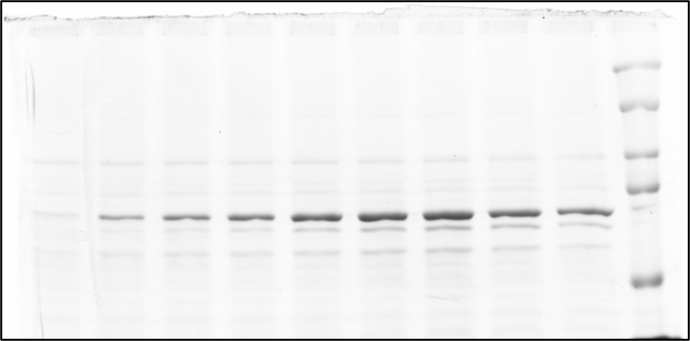
\includegraphics[width=0.94\linewidth, height=3.5cm, keepaspectratio]{figures_opt/image29.png}};
        \foreach \lbl/\xpos in {E11/-2.65, E12/-2.08, E13/-1.52, E14/-0.95, E15/-0.38, E16/0.18, E17/0.75, E18/1.32, E19/1.88, M/2.48} {
          \node[anchor=south, font=\tiny\bfseries\color{steelsecondary}] at ([xshift=\xpos cm, yshift=0.04cm]secgel.north) {\lbl};
        }
      \end{tikzpicture}\\[0.3em]
      \begin{block}{}
        \scriptsize Homogeneous, single-band DDX3X ($\sim 73\text{ kDa}$) recovered across peak fractions E13--E18, suitable for downstream EMSA assays.
      \end{block}
    \end{column}

    \begin{column}{0.49\textwidth}
      \centering
      \textbf{\small\color{navyprimary} UV Absorbance ($A_{280}$) Chromatogram}\\[0.25em]
      \figbox[width=0.95\linewidth, height=4.8cm, keepaspectratio]{figures_opt/image28.png}\\[0.2em]
      {\scriptsize\color{textmuted} Sharp elution peak at $\sim 13.5\text{ mL}$ (blue trace) overlaid with molecular weight standards (red dotted trace).}
    \end{column}
  \end{columns}
\end{frame}

% ==============================================================================
% SLIDE 13: OBJECTIVE 2 - IN VITRO TRANSCRIPTION METHODOLOGY
% ==============================================================================
\begin{frame}{Objective 2: In Vitro Transcription (IVT)}
  \framesubtitle{Methodology}
  \begin{columns}[c]
    \begin{column}{0.58\textwidth}
      \begin{block}{Cloning, Screening \& RNA Synthesis Workflow}
        \footnotesize
        \begin{enumerate}
          \setlength\itemsep{0.35em}
          \item \textbf{Transformation \& Selection:} Recombinant plasmids carrying Influenza B virus gene segments were transformed into competent \textit{E.\ coli} cells and selected on antibiotic-containing agar plates.
          \item \textbf{Colony PCR Screening:} Positive recombinant clones were identified via colony PCR (CMV-F / BGH-R primers) and verified by agarose gel electrophoresis.
          \item \textbf{DNA Template Preparation:} Verified plasmids served as templates for PCR amplification of mini-IVT constructs.
          \item \textbf{T7 In Vitro Transcription:} T7 RNA polymerase transcribed the DNA templates \textit{in vitro} to generate viral RNA segments.
          \item \textbf{Downstream Application:} Synthesized RNA was purified and used for RNA--protein interaction studies.
        \end{enumerate}
      \end{block}
    \end{column}

    \begin{column}{0.39\textwidth}
      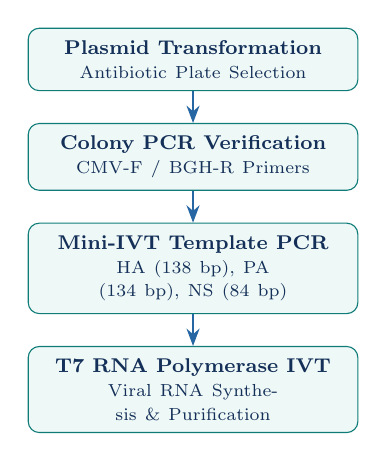
\begin{tikzpicture}[
        scale=0.9, transform shape,
        node distance=0.45cm,
        pbox/.style={draw=biotechteal, fill=tealbg, rounded corners=4pt, text width=4.3cm, align=center, inner sep=5pt, font=\footnotesize\bfseries\color{navyprimary}},
        arr/.style={-{Stealth[length=2.2mm]}, thick, steelsecondary}
      ]
        \node[pbox] (a) {Plasmid Transformation\\{\normalfont\scriptsize Antibiotic Plate Selection}};
        \node[pbox, below=of a] (b) {Colony PCR Verification\\{\normalfont\scriptsize CMV-F / BGH-R Primers}};
        \node[pbox, below=of b] (c) {Mini-IVT Template PCR\\{\normalfont\scriptsize HA (138 bp), PA (134 bp), NS (84 bp)}};
        \node[pbox, below=of c] (d) {T7 RNA Polymerase IVT\\{\normalfont\scriptsize Viral RNA Synthesis \& Purification}};
        \draw[arr] (a) -- (b);
        \draw[arr] (b) -- (c);
        \draw[arr] (c) -- (d);
      \end{tikzpicture}
    \end{column}
  \end{columns}
\end{frame}

% ==============================================================================
% SLIDE 14: PCR AMPLIFICATION FOR MINI IVT TEMPLATE GENERATION
% ==============================================================================
\begin{frame}{PCR Amplification for Mini IVT Template Generation}
  \begin{columns}[c]
    \begin{column}{0.46\textwidth}
      \centering
      \textbf{\small\color{navyprimary} Agarose Gel Electrophoresis of Mini Templates}\\[0.3em]
      \begin{columns}[T]
        \begin{column}{0.48\textwidth}
          \centering
          {\scriptsize\bfseries 1kb \hspace{0.15cm} PA \hspace{0.15cm} HA}\\
          \figbox[height=3.5cm, keepaspectratio]{figures_opt/image30.png}\\
          {\scriptsize\color{steelsecondary}\textbf{B mini PA:} 134 bp}\\
          {\scriptsize\color{steelsecondary}\textbf{B mini HA:} 138 bp}
        \end{column}
        \begin{column}{0.48\textwidth}
          \centering
          {\scriptsize\bfseries 1kb \hspace{0.25cm} NS}\\
          \figbox[height=3.5cm, keepaspectratio]{figures_opt/image31.png}\\
          {\scriptsize\color{steelsecondary}\textbf{B mini NS:} 84 bp}
        \end{column}
      \end{columns}
    \end{column}

    \begin{column}{0.52\textwidth}
      \centering
      \textbf{\small\color{navyprimary} Transformation Plates ($-\text{ve}$ vs.\ $+\text{ve}$ Controls)}\\[0.25em]
      {\scriptsize\bfseries HA $-\text{ve}$ \hspace{1.8cm} HA $+\text{ve}$}\\
      \figbox[height=1.5cm, keepaspectratio]{figures_opt/image34.png}\\[0.2em]
      {\scriptsize\bfseries PA $-\text{ve}$ \hspace{1.8cm} PA $+\text{ve}$}\\
      \figbox[height=1.5cm, keepaspectratio]{figures_opt/image32.png}\\[0.2em]
      {\scriptsize\bfseries NS $-\text{ve}$ \hspace{1.8cm} NS $+\text{ve}$}\\
      \figbox[height=1.5cm, keepaspectratio]{figures_opt/image33.png}
    \end{column}
  \end{columns}
\end{frame}

% ==============================================================================
% SLIDE 15: COLONY PCR & MASTER PLATES
% ==============================================================================
\begin{frame}{Colony PCR Screening \& Master Plates}
  \begin{columns}[c]
    \begin{column}{0.36\textwidth}
      \centering
      \textbf{\small\color{navyprimary} Colony PCR (CMV-F / BGH-R)}\\[0.2em]
      {\scriptsize\color{textmuted} Lanes: $-\text{ve}$, $+\text{ve}$, Clones 1--6}\\[0.2em]
      \figbox[height=4.6cm, keepaspectratio]{figures_opt/image35.png}\\[0.2em]
      {\scriptsize\color{steelsecondary} Top: \textbf{B mini HA} \& \textbf{NS} $\cdot$ Bottom: \textbf{B mini PA}}
    \end{column}

    \begin{column}{0.62\textwidth}
      \centering
      \textbf{\small\color{navyprimary} Master Plates of Verified Transformants}\\[0.35em]
      \begin{columns}[c]
        \begin{column}{0.54\textwidth}
          \centering
          \figbox[width=0.94\linewidth, height=3.6cm, keepaspectratio]{figures_opt/image36.png}\\[0.25em]
          {\scriptsize\bfseries\color{navyprimary} PA (Left) \hspace{1.0cm} HA (Right)}
        \end{column}
        \begin{column}{0.42\textwidth}
          \centering
          \figbox[width=0.90\linewidth, height=3.6cm, keepaspectratio]{figures_opt/image37.png}\\[0.25em]
          {\scriptsize\bfseries\color{navyprimary} NS Master Plate}
        \end{column}
      \end{columns}
    \end{column}
  \end{columns}
\end{frame}

% ==============================================================================
% SLIDE 16: IN-VITRO TRANSCRIPTION
% ==============================================================================
\begin{frame}{In-Vitro Transcription (IVT) \& RNA Purification}
  \begin{columns}[c]
    \begin{column}{0.98\textwidth}
      \centering
      \textbf{\small\color{navyprimary} T7 RNA Polymerase Transcription Mechanism}\\[0.2em]
      \figbox[width=0.78\linewidth, height=2.55cm, keepaspectratio]{figures_opt/image39.png}\\[0.3em]
      \textbf{\small\color{biotechteal} TRIzol--Chloroform RNA Extraction \& Precipitation Workflow}\\[0.2em]
      \figbox[width=0.82\linewidth, height=2.55cm, keepaspectratio]{figures_opt/image38.png}
    \end{column}
  \end{columns}
\end{frame}

% ==============================================================================
% SLIDE 17: OBJECTIVE 3 - EMSA METHODOLOGY
% ==============================================================================
\begin{frame}{Objective 3: Electrophoretic Mobility Shift Assay (EMSA)}
  \framesubtitle{Methodology}
  \begin{columns}[T]
    \begin{column}{0.52\textwidth}
      \begin{block}{Experimental Protocol}
        \footnotesize
        \begin{enumerate}
          \setlength\itemsep{0.4em}
          \item \textbf{Binding Reaction Assembly:} Purified recombinant DDX3X (titrated $0\text{--}20\ \mu\text{M}$) was incubated with \textit{in vitro} transcribed radiolabelled Influenza B virus RNA.
          \item \textbf{Complex Formation:} Protein--RNA binding reactions were equilibrated to allow ribonucleoprotein complex formation.
          \item \textbf{Native PAGE Resolution:} Reaction mixtures were resolved on a non-denaturing native polyacrylamide gel to preserve intact protein--RNA interactions.
          \item \textbf{Mobility Shift Analysis:} Protein--RNA complexes exhibit reduced electrophoretic mobility compared to free RNA, enabling direct assessment of binding.
        \end{enumerate}
      \end{block}
    \end{column}

    \begin{column}{0.45\textwidth}
      \begin{exampleblock}{Biophysical Principle}
        \footnotesize
        \begin{itemize}
          \item \textbf{Free RNA:} Low molecular weight and high negative charge-to-mass ratio $\rightarrow$ migrates rapidly toward the anode ($+$).
          \item \textbf{DDX3X--RNA Complex:} Larger hydrodynamic radius and reduced net charge density $\rightarrow$ retarded migration (\textbf{Bound RNA shift}).
        \end{itemize}
      \end{exampleblock}
      \vspace{0.2cm}
      \begin{alertblock}{Titration Range Tested}
        \centering\small\bfseries $0,\ 0.5,\ 1,\ 3,\ 5,\ 10,\ 15,\ 20\ \mu\text{M}$ DDX3X
      \end{alertblock}
    \end{column}
  \end{columns}
\end{frame}

% ==============================================================================
% SLIDE 18: ELECTROPHORETIC MOBILITY SHIFT ASSAY SCHEMATIC
% ==============================================================================
\begin{frame}{Electrophoretic Mobility Shift Assay: Principle \& Workflow}
  \begin{columns}[c]
    \begin{column}{0.50\textwidth}
      \centering
      \textbf{\small\color{navyprimary} Native Gel Electrophoresis Setup}\\[0.2em]
      \figbox[width=0.92\linewidth, height=5.2cm, keepaspectratio]{figures_opt/image40.png}
    \end{column}

    \begin{column}{0.48\textwidth}
      \centering
      \textbf{\small\color{navyprimary} Step-by-Step EMSA Workflow}\\[0.2em]
      \figbox[width=0.88\linewidth, height=5.2cm, keepaspectratio]{figures_opt/image41.png}
    \end{column}
  \end{columns}
\end{frame}

% ==============================================================================
% SLIDE 19: EMSA OF DDX3X WITH PB1 AND PB2 IBV SEGMENTS
% ==============================================================================
\begin{frame}{EMSA of DDX3X with PB1 and PB2 Influenza B Virus Segments}
  \begin{columns}[c]
    \begin{column}{0.48\textwidth}
      \centering
      {\normalsize\bfseries\color{navyprimary} PB1 Segment}\\[0.1em]
      {\scriptsize\color{textdark}\textbf{Protein Concentration ($\mu$M)}}\\[0.15em]
      \begin{tikzpicture}
        \node[draw=slateborder, inner sep=2pt, fill=black] (gel1) {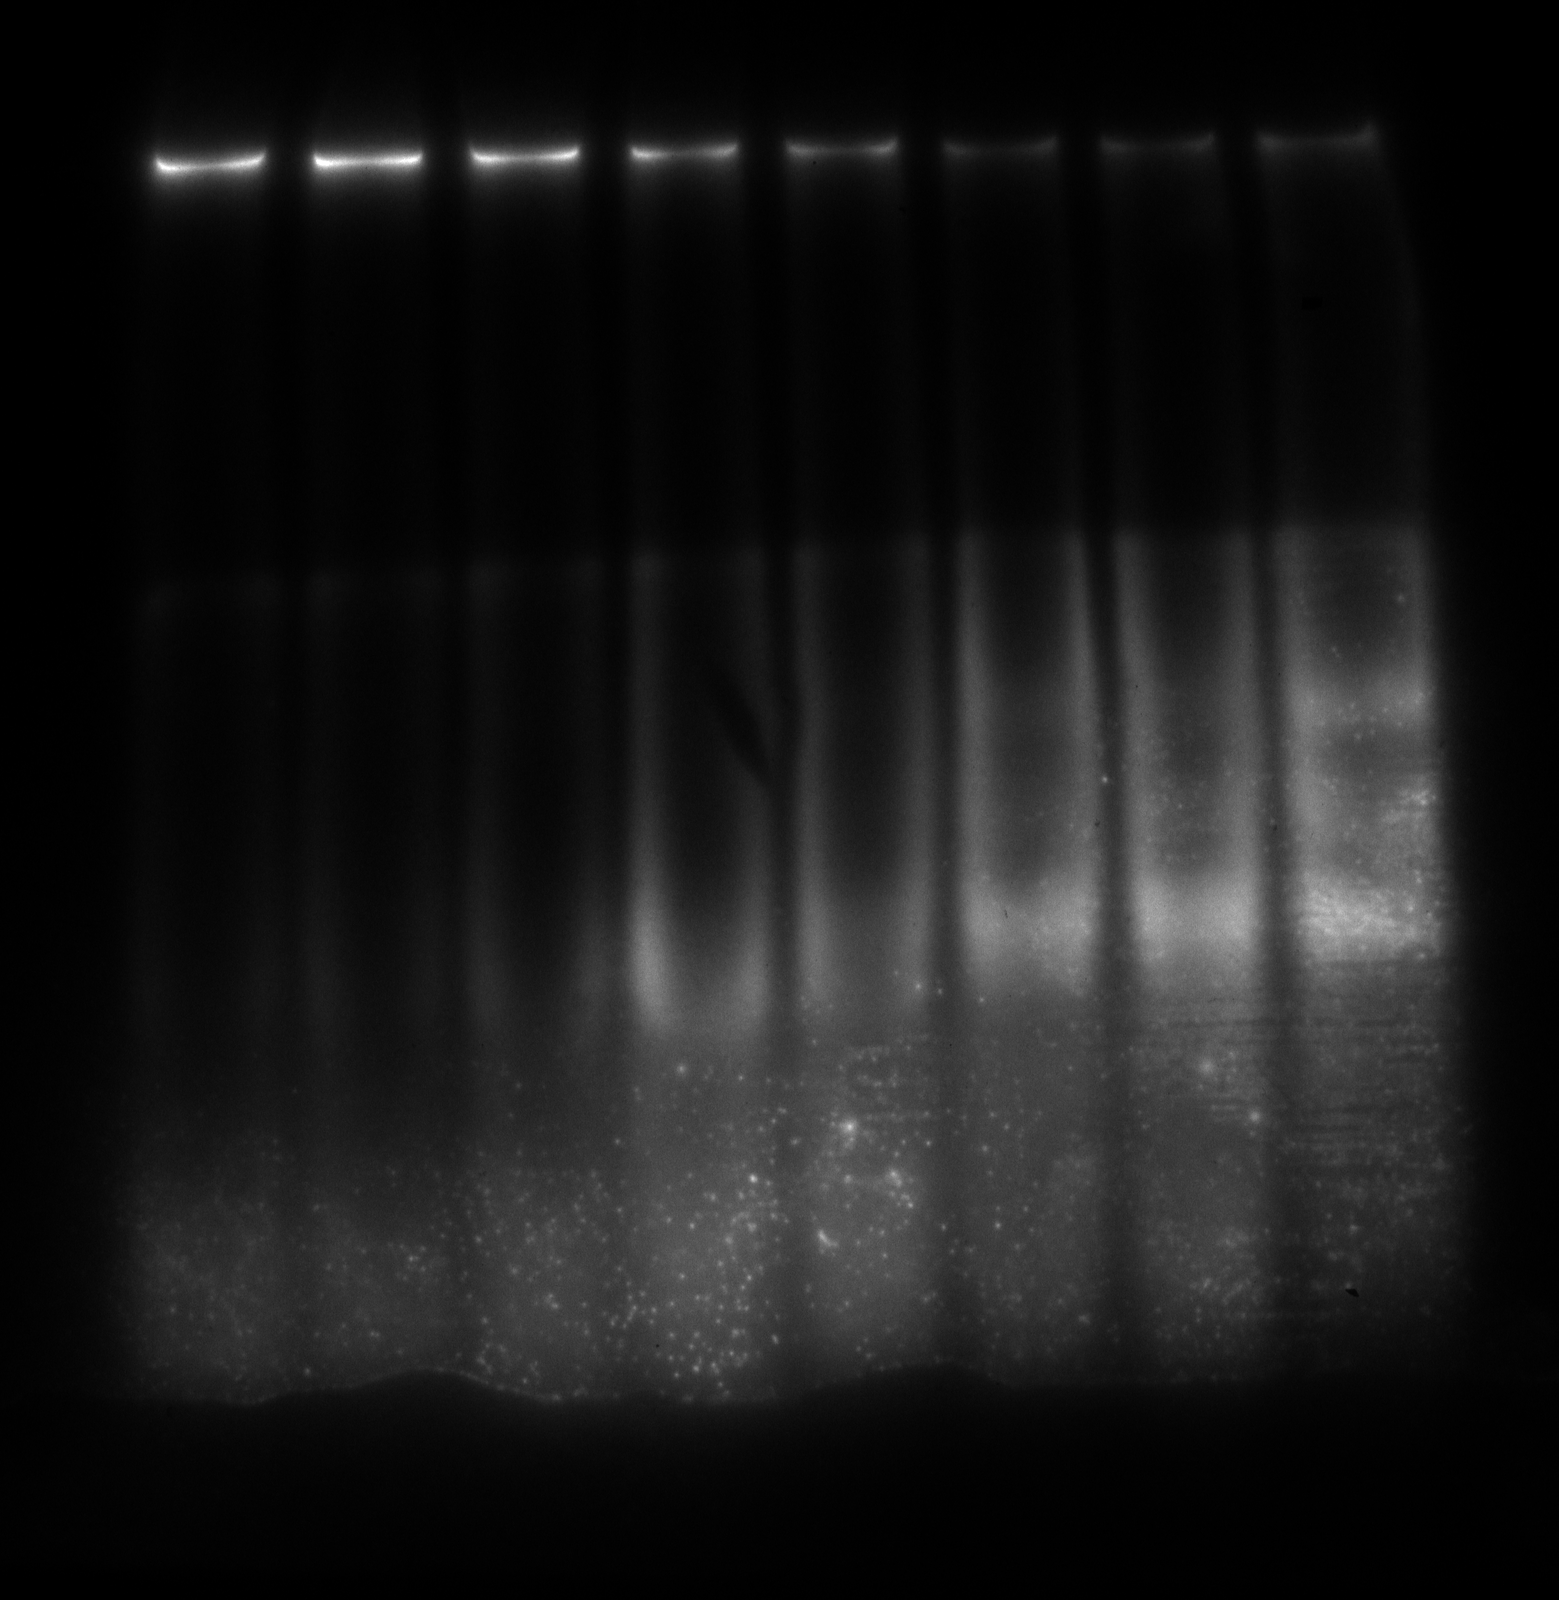
\includegraphics[height=3.8cm, keepaspectratio]{figures_opt/image42.png}};
        \foreach \conc/\xpos in {20/-1.32, 15/-0.93, 10/-0.54, 5/-0.15, 3/0.24, 1/0.63, 0.5/1.02, 0/1.41} {
          \node[anchor=south, font=\tiny\bfseries\color{navyprimary}] at ([xshift=\xpos cm, yshift=0.04cm]gel1.north) {\conc};
        }
        \node[anchor=west, font=\scriptsize\bfseries\color{crimsonalert}] at ([xshift=0.12cm, yshift=1.3cm]gel1.east) {$\leftarrow$ Bound RNA};
        \node[anchor=west, font=\scriptsize\bfseries\color{biotechteal}] at ([xshift=0.12cm, yshift=-0.5cm]gel1.east) {$\leftarrow$ Unbound RNA};
      \end{tikzpicture}
    \end{column}

    \begin{column}{0.48\textwidth}
      \centering
      {\normalsize\bfseries\color{navyprimary} PB2 Segment}\\[0.1em]
      {\scriptsize\color{textdark}\textbf{Protein Concentration ($\mu$M)}}\\[0.15em]
      \begin{tikzpicture}
        \node[draw=slateborder, inner sep=2pt, fill=black] (gel2) {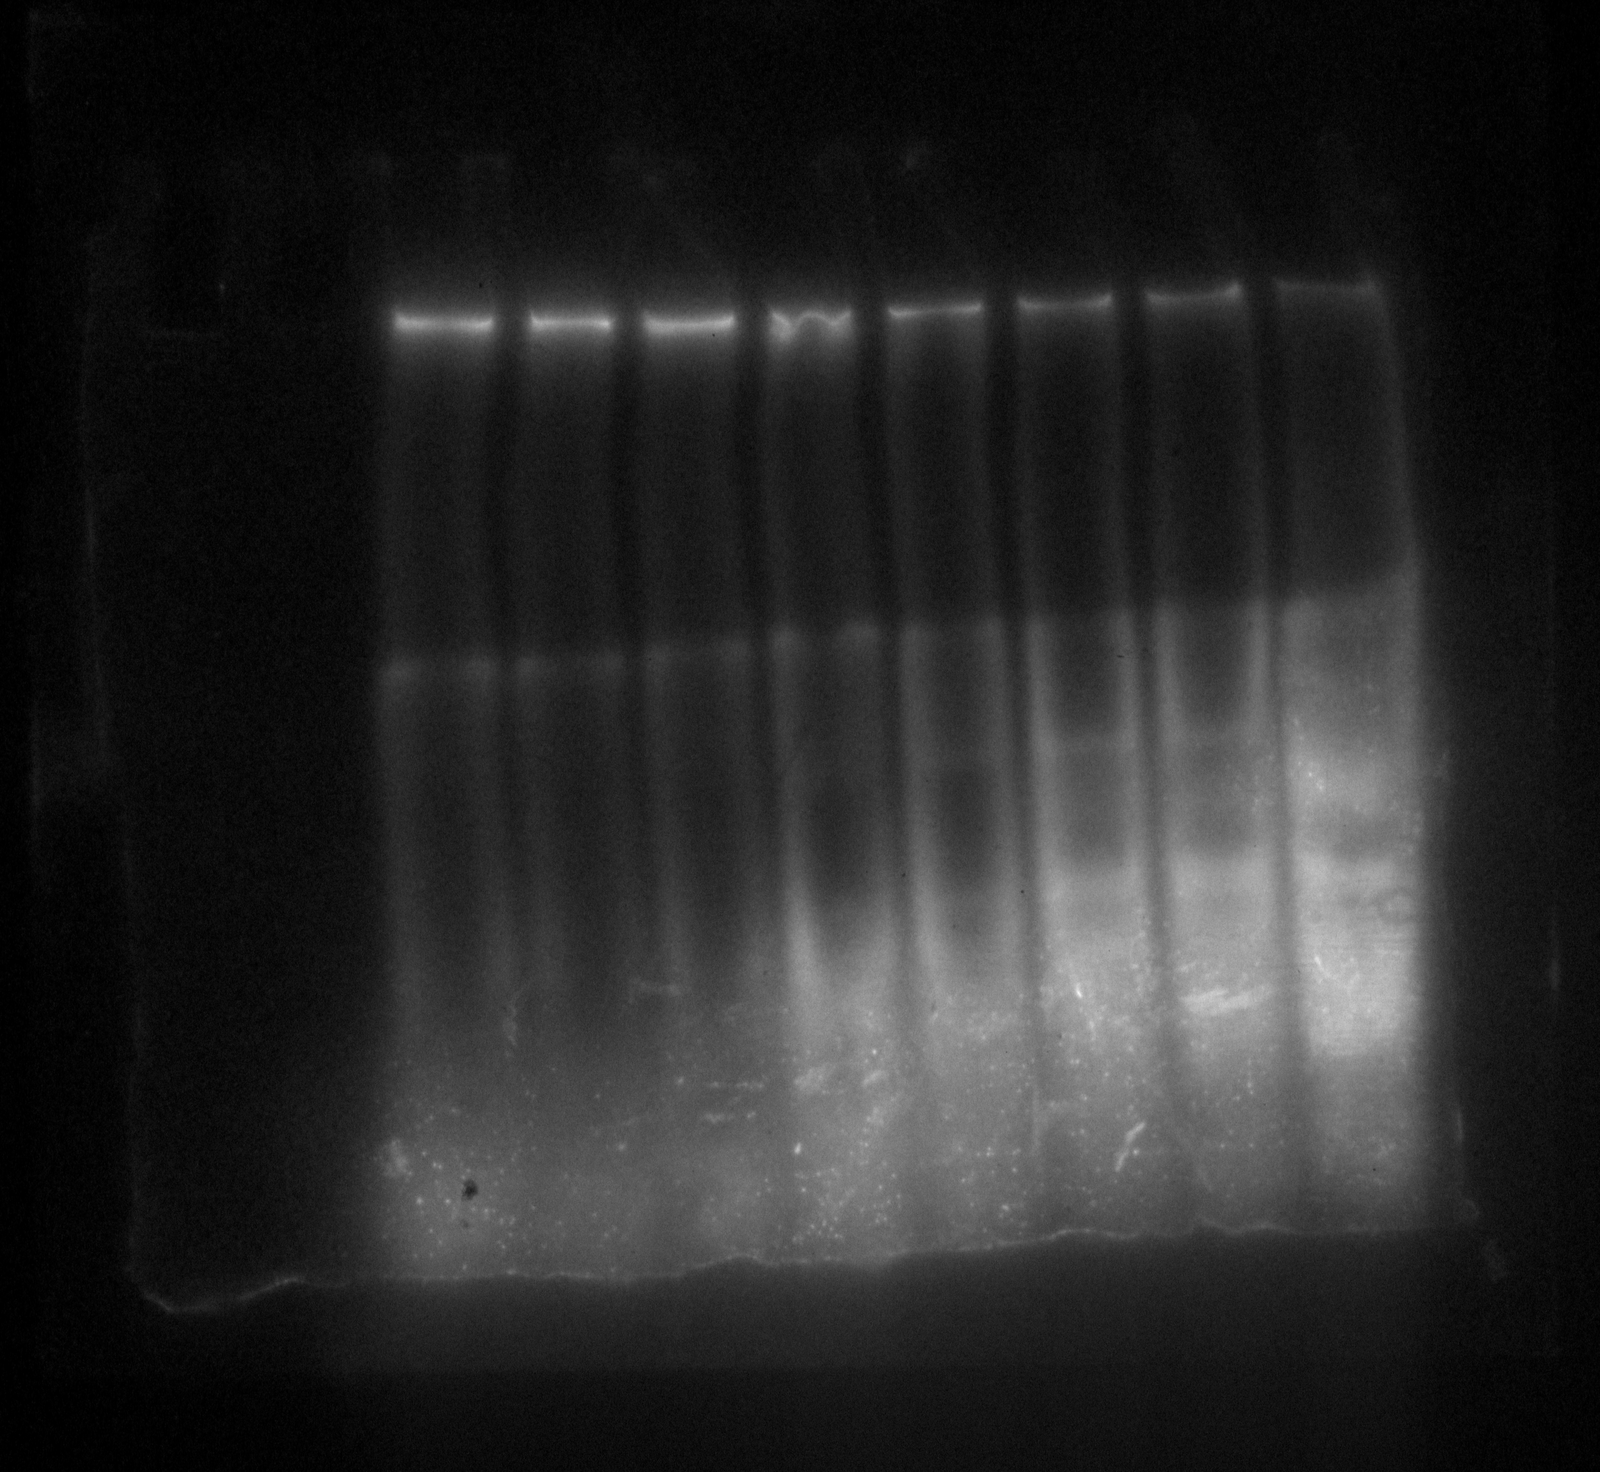
\includegraphics[height=3.8cm, keepaspectratio]{figures_opt/image43.png}};
        \foreach \conc/\xpos in {20/-0.95, 15/-0.61, 10/-0.27, 5/0.07, 3/0.41, 1/0.75, 0.5/1.09, 0/1.43} {
          \node[anchor=south, font=\tiny\bfseries\color{navyprimary}] at ([xshift=\xpos cm, yshift=0.04cm]gel2.north) {\conc};
        }
        \node[anchor=west, font=\scriptsize\bfseries\color{crimsonalert}] at ([xshift=0.12cm, yshift=1.2cm]gel2.east) {$\leftarrow$ Bound RNA};
        \node[anchor=west, font=\scriptsize\bfseries\color{biotechteal}] at ([xshift=0.12cm, yshift=-0.6cm]gel2.east) {$\leftarrow$ Unbound RNA};
      \end{tikzpicture}
    \end{column}
  \end{columns}

  \vspace{0.15cm}
  \begin{center}
    \begin{block}{}
      \centering\footnotesize\textbf{Key Observation:} Concentration-dependent mobility shift confirms direct physical binding of recombinant DDX3X to both \textbf{PB1} and \textbf{PB2} genomic RNA segments of Influenza B virus.
    \end{block}
  \end{center}
\end{frame}

% ==============================================================================
% SLIDE 20: SUMMARY AND FUTURE DIRECTIONS
% ==============================================================================
\begin{frame}{Summary and Future Directions}
  \begin{columns}[T]
    \begin{column}{0.52\textwidth}
      \begin{block}{Summary of Work Accomplished}
        \begin{itemize}
          \setlength\itemsep{0.5em}
          \item Expressed and purified recombinant His-tagged \textbf{DDX3X} protein using \textbf{Ni-NTA affinity chromatography} followed by \textbf{size-exclusion chromatography (SEC)}.
          \item Characterized purified DDX3X ($\sim 73\text{ kDa}$) via \textbf{SDS-PAGE} and prepared reagents for RNA--protein interaction assays.
          \item Cloned and verified Influenza B viral gene segments (\textbf{HA, PA, NS}) using \textbf{colony PCR} and agarose gel electrophoresis.
          \item Demonstrated direct, concentration-dependent binding between host RNA helicase \textbf{DDX3X} and Influenza B virus \textbf{PB1} and \textbf{PB2} RNA segments via \textbf{EMSA}.
        \end{itemize}
      \end{block}
    \end{column}

    \begin{column}{0.45\textwidth}
      \begin{exampleblock}{Future Directions}
        \begin{itemize}
          \setlength\itemsep{0.65em}
          \item \textbf{Complete Segment Panel:} Generation of the remaining individual genomic RNA segments of Influenza B virus \textit{in vitro} (NP, NA, M, HA, PA, NS).
          \item \textbf{Comprehensive Binding Profiling:} Characterizing the interaction and binding affinity ($K_d$) between DDX3X and each of the 8 Influenza B virus genomic RNA segments \textit{in vitro}.
          \item \textbf{Mechanistic Validation:} Mapping specific RNA motifs recognized by DDX3X and assessing functional impact on viral polymerase activity.
        \end{itemize}
      \end{exampleblock}
    \end{column}
  \end{columns}
\end{frame}

\begin{frame}{Acknowledgments}
  \begin{center}
    {\Huge\bfseries\color{navyprimary} Thank You}
  \end{center}
  \vspace{0.25cm}
  \begin{block}{Gratitude \& Mentorship}
    \small
    I would like to express my sincere gratitude to \textbf{Prof.\ Arindam Mondal}, my Principal Investigator, for giving me the opportunity to work in the \textbf{Molecular Virology Laboratory} at IIT Kharagpur. His invaluable guidance, constant encouragement, insightful suggestions, and unwavering support have been instrumental throughout the course of this internship and have greatly enriched my learning experience.
  \end{block}
  \vspace{0.2cm}
  \begin{exampleblock}{Molecular Virology Laboratory}
    \small
    I am also deeply thankful to all the members of the \textbf{Molecular Virology Laboratory} (including Mr.\ Soumik Dey) for their continuous support, technical guidance, constructive discussions, and for creating a collaborative and inspiring research environment. Their willingness to share their knowledge and expertise has contributed significantly to both my academic and practical understanding of molecular virology.
  \end{exampleblock}
\end{frame}

\end{document}
